% Options for packages loaded elsewhere
\PassOptionsToPackage{unicode}{hyperref}
\PassOptionsToPackage{hyphens}{url}
%
\documentclass[
]{article}
\usepackage{lmodern}
\usepackage{amssymb,amsmath}
\usepackage{ifxetex,ifluatex}
\ifnum 0\ifxetex 1\fi\ifluatex 1\fi=0 % if pdftex
  \usepackage[T1]{fontenc}
  \usepackage[utf8]{inputenc}
  \usepackage{textcomp} % provide euro and other symbols
\else % if luatex or xetex
  \usepackage{unicode-math}
  \defaultfontfeatures{Scale=MatchLowercase}
  \defaultfontfeatures[\rmfamily]{Ligatures=TeX,Scale=1}
\fi
% Use upquote if available, for straight quotes in verbatim environments
\IfFileExists{upquote.sty}{\usepackage{upquote}}{}
\IfFileExists{microtype.sty}{% use microtype if available
  \usepackage[]{microtype}
  \UseMicrotypeSet[protrusion]{basicmath} % disable protrusion for tt fonts
}{}
\makeatletter
\@ifundefined{KOMAClassName}{% if non-KOMA class
  \IfFileExists{parskip.sty}{%
    \usepackage{parskip}
  }{% else
    \setlength{\parindent}{0pt}
    \setlength{\parskip}{6pt plus 2pt minus 1pt}}
}{% if KOMA class
  \KOMAoptions{parskip=half}}
\makeatother
\usepackage{xcolor}
\IfFileExists{xurl.sty}{\usepackage{xurl}}{} % add URL line breaks if available
\IfFileExists{bookmark.sty}{\usepackage{bookmark}}{\usepackage{hyperref}}
\hypersetup{
  hidelinks,
  pdfcreator={LaTeX via pandoc}}
\urlstyle{same} % disable monospaced font for URLs
\usepackage{graphicx}
\makeatletter
\def\maxwidth{\ifdim\Gin@nat@width>\linewidth\linewidth\else\Gin@nat@width\fi}
\def\maxheight{\ifdim\Gin@nat@height>\textheight\textheight\else\Gin@nat@height\fi}
\makeatother
% Scale images if necessary, so that they will not overflow the page
% margins by default, and it is still possible to overwrite the defaults
% using explicit options in \includegraphics[width, height, ...]{}
\setkeys{Gin}{width=\maxwidth,height=\maxheight,keepaspectratio}
% Set default figure placement to htbp
\makeatletter
\def\fps@figure{htbp}
\makeatother
\setlength{\emergencystretch}{3em} % prevent overfull lines
\providecommand{\tightlist}{%
  \setlength{\itemsep}{0pt}\setlength{\parskip}{0pt}}
\setcounter{secnumdepth}{-\maxdimen} % remove section numbering
\ifluatex
  \usepackage{selnolig}  % disable illegal ligatures
\fi

\author{}
\date{}

\begin{document}

\hypertarget{uxe9tude-du-robot-trooper}{%
\section{Étude du robot TROOPER}\label{uxe9tude-du-robot-trooper}}

\hypertarget{partie-i---probluxe9matique-et-objectif}{%
\subsection{Partie I - Problématique et
objectif}\label{partie-i---probluxe9matique-et-objectif}}

En culture hors-sol (\textbf{figure 1}), il faut constamment déplacer
les pots pour profiter de la lumière, pour regrouper les cultures,
isoler celles qui posent problème, ... Ce travail est pénible
physiquement et les pépiniéristes peinent à trouver de la main d'œuvre
pour réaliser ces tâches quotidiennes difficiles.

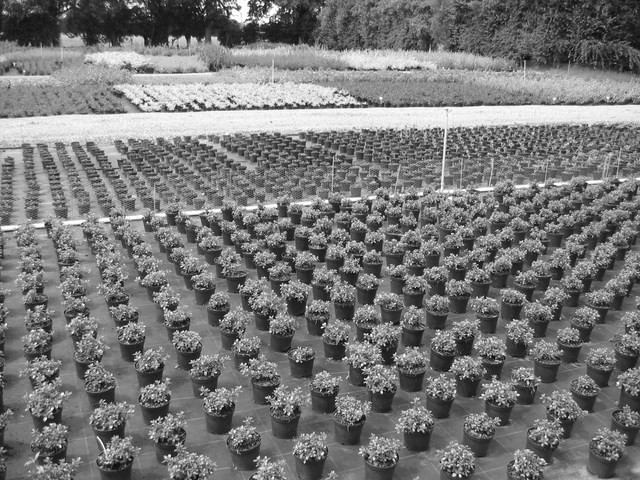
\includegraphics[width=5.91531in,height=1.96921in]{media/image1.jpg}

\textbf{Figure 1 -} Exemple de culture hors-sol \textbf{Figure 2 -}
Robot TROOPER de la société

\hypertarget{instar-robotics}{%
\subsubsection{INSTAR ROBOTICS}\label{instar-robotics}}

La Startup INSTAR ROBOTICS, spécialisée dans le développement de robots
d'assistance, a conçu le robot TROOPER qui permet de répondre à ce
besoin (\textbf{figure 2}).

L'objectif du travail proposé dans cette épreuve est de justifier les
solutions techniques retenues par la société INSTAR ROBOTICS dans le but
de respecter le cahier des charges élaboré en partenariat avec des
pépiniéristes.

\hypertarget{partie-ii---cahier-des-charges}{%
\subsection{Partie II - Cahier des
charges}\label{partie-ii---cahier-des-charges}}

Les spécifications que doit respecter le robot sont directement liées
aux contraintes imposées par la culture hors-sol.

Une des contraintes majeures est la vitesse à laquelle le robot doit se
déplacer et réaliser les opérations de prise/dépose de pots afin d'être
si possible aussi rapide qu'une personne.

Un exemple de tâche à réaliser consiste à déplacer 4 rangées de 6 pots
d'une zone à une autre. Le robot doit prendre les 6 pots de la rangée 1
de la zone 1, puis les déplacer dans la rangée 1 de la zone 2, de même
pour les autres rangées.

On note \emph{T\textsubscript{p }}le temps de prise d'une rangée de 6
pots, égal au temps de dépose (ce temps inclut toutes les manœuvres et
est estimé à 30 s). On suppose que le robot se déplace à la vitesse
constante \emph{V} en ligne droite sur une distance \emph{L} = 10m
séparant les rangées de chaque zone (\textbf{figure 3}). La distance
entre deux rangées d'une zone est notée \(\mathcal{l}\) = 50cm.

\hypertarget{figure-3---tuxe2che-uxe0-effectuer-par-le-robot}{%
\subsubsection{\texorpdfstring{\textbf{Figure 3 -} Tâche à effectuer par
le
robot}{Figure 3 - Tâche à effectuer par le robot}}\label{figure-3---tuxe2che-uxe0-effectuer-par-le-robot}}

Un employé qui utilise un chariot à pousser (pour déplacer 6 pots à
chaque fois) met un temps total \emph{T\textsubscript{m} pour} réaliser
cette tâche de repositionnement de 4 rangées de pots.

\textbf{Q1.} Déterminer la vitesse \emph{V}, supposée constante, à
laquelle doit se déplacer le robot en ligne droite pour réaliser la
tâche au maximum en \emph{T\textsubscript{m }}secondes en fonction de
\emph{L}, \(\mathcal{l}\), \emph{T\textsubscript{m }}et
\emph{T\textsubscript{p}}. Faire l'application numérique pour une durée
\emph{T\textsubscript{m }}de 320 secondes.

Les autres éléments du cahier des charges pourraient être justifiés de
la même manière. Le diagramme des exigences de la \textbf{figure 4}
liste les éléments principaux utiles pour le dimensionnement du robot.

Le robot est constitué de plusieurs chaînes d'énergie et d'information.
Nous analyserons dans un premier temps les chaînes d'énergie et
d'information relatives au déplacement du robot, puis, dans un second
temps, celles relatives à la prise et dépose des pots.

Pour se déplacer, le robot utilise deux roues motorisées indépendantes à
l'avant et deux roues folles à l'arrière. Le robot embarque une batterie
pouvant délivrer jusqu'à 100 Volts. Une carte de commande dédiée à
chaque moteur utilise l'information d'un codeur incrémental monté sur
chaque axe moteur pour donner des ordres au hacheur pilotant ce même
moteur. Un réducteur permet d'adapter la vitesse de rotation du moteur
pour la transmettre à la roue. Pour permettre au robot de se diriger
correctement, un dispositif LIDAR (Laser Imaging Detection And Ranging :
émetteur/récepteur infrarouge) fournit des informations sur
l'environnement à un micro-ordinateur qui se charge d'envoyer des
consignes aux cartes de commande des moteurs. L'utilisateur peut
communiquer avec le robot à l'aide d'une tablette en Bluetooth.

\textbf{Q2.} À l'aide des informations ci-dessus, compléter les chaînes
d'énergie et d'information pour le déplacement du robot.


\includegraphics[width=6.56333in,height=4.01667in]{media/image3.png}

\textbf{Figure 4 -} Diagramme des exigences du robot Trooper

\hypertarget{partie-iii---duxe9placement-du-robot}{%
\subsection{Partie III - Déplacement du
robot}\label{partie-iii---duxe9placement-du-robot}}

Nous allons montrer tout d'abord la nécessité d'asservir en vitesse les
moteurs pour assurer un déplacement correct du robot.

\textbf{III.1 - Nécessité d'un asservissement en vitesse}

Chaque roue motorisée du robot a pour rayon \emph{r} = 15cm et le
rapport de réduction du réducteur associé à chaque moteur vaut
\emph{k\textsubscript{r }}= 1/40 .

Les caractéristiques d'un moteur sont :

\begin{itemize}
\item
  \begin{quote}
  \emph{J\textsubscript{m}} = 3,4.10\textsuperscript{-3} kg.m² moment
  d'inertie de l'ensemble motoréducteur ramené sur l'arbre moteur,
  \end{quote}
\item
  \begin{quote}
  \emph{k\textsubscript{m}} = 0,2 N.m.A\textsuperscript{-1} constante de
  couple (égale à la constante de vitesse)
  \end{quote}
\item
  \begin{quote}
  \emph{R\textsubscript{m}} = 1 Ω résistance interne du moteur
  \end{quote}
\item
  \begin{quote}
  vitesse maximale du moteur égale à 3000tr·min−\textsuperscript{1}.
  \end{quote}
\end{itemize}

\textbf{Q3.} Vérifier que les éléments choisis permettent de respecter
le critère de vitesse maximale défini dans le diagramme des exigences.

On souhaite que le robot se déplace selon une loi trapèze de vitesse
avec \emph{V\textsubscript{max }}la vitesse maximale du robot (du
diagramme des exigences) pour parcourir une distance \emph{D} = 10m. On
donne le temps total \emph{T} = 10s et on cherche la durée
d'accélération égale à la durée de décélération δ\emph{t}. Pour la
question suivante, on suppose, de manière simplifiée, que le robot suit
parfaitement cette consigne.

\textbf{Q4.} Déterminer l'expression du temps δ\emph{t} pour respecter
le déplacement souhaité en fonction de \emph{D}, \emph{T} et
\emph{V\textsubscript{max}}. Faire l'application numérique.

On suppose que les deux moteurs sont identiques. Les équations qui
caractérisent le comportement en ligne droite du robot sont les
suivantes :

\begin{itemize}
\item
  \(u_{m}\left( t \right) = R_{m}.i_{m}\left( t \right) + k_{m}.\omega_{m}\left( t \right)\)
  (1)
\item
  \({2C}_{m}\left( t \right) - C_{r}\left( t \right) = J.\frac{d\omega_{m}\left( t \right)}{\text{dt}}\)
  (2)
\item
  \(C_{m}\left( t \right) = k_{m}.i_{m}\left( t \right)\) (3)
\item
  \(v\left( t \right) = k_{t}.\omega_{m}\left( t \right)\) (4)
\end{itemize}

où \(\omega_{m}\left( t \right)\) est la vitesse angulaire d'un moteur,
\(u_{m}\left( t \right)\) la tension de commande d'un moteur,
\(i_{m}\left( t \right)\) le courant traversant chaque moteur et
\(C_{m}\left( t \right)\) le couple exercé par un moteur.

\emph{C\textsubscript{r}}(\emph{t}) est un couple résistant global
supposé nul dans un premier temps pour \textbf{Q5} et \textbf{Q6}.
\emph{J} est le moment d'inertie équivalent de l'ensemble en mouvement
ramené sur un arbre moteur. \(v\left( t \right)\) est la vitesse du
robot en ligne droite par rapport au sol.

\textbf{Q5.} Déterminer l'équation différentielle vérifiée par
\(v\left( t \right)\) avec \(u_{m}\left( t \right)\) comme entrée.

Vérifier que
\(v\left( t \right) = \alpha_{0}(t - \tau_{m} + \tau_{m}e^{- t/\tau_{m}})\)
est solution de l'équation différentielle pour une consigne de tension
\(u_{m}\left( t \right) = \frac{u_{0}}{\text{δt}}t.u(t)\) où
\(u\left( t \right)\) est un échelon unitaire.

On suppose que \emph{v}(0) = 0.

On donnera l'expression de \(\alpha_{0}\) et \(\tau_{m}\) en fonction de
\(u_{0}\), \(\text{δt}\) et des constantes intervenant dans les
équations du moteur.

La \textbf{figure 5} montre la réponse du robot à une tension de
commande en trapèze. La courbe de vitesse simulée est tracée ainsi que
la courbe de vitesse de consigne fournie.

\textbf{Q6.} En s'aidant de l'expression de la vitesse donnée
précédemment, estimer la valeur de \(\tau_{m}\) à partir de la courbe de
vitesse réelle. Faire apparaître le tracé sur la figure du
\textbf{Document Réponse}.

Au regard des simulations effectuées, on constate qu'on peut confondre
la vitesse de consigne avec la vitesse simulée et ainsi travailler
directement avec le profil de vitesse de consigne pour des études
cinématiques.

Le robot évolue sur un terrain souvent boueux et accidenté, ce qui
engendre des perturbations sur les roues, le robot ne se déplace alors
plus à la vitesse souhaitée. De plus, pour des courants trop faibles,
les roues ne tournent pas à cause des frottements. La vitesse de
déplacement du robot est donc asservie à une vitesse de consigne notée
\(v_{c}(t)\)

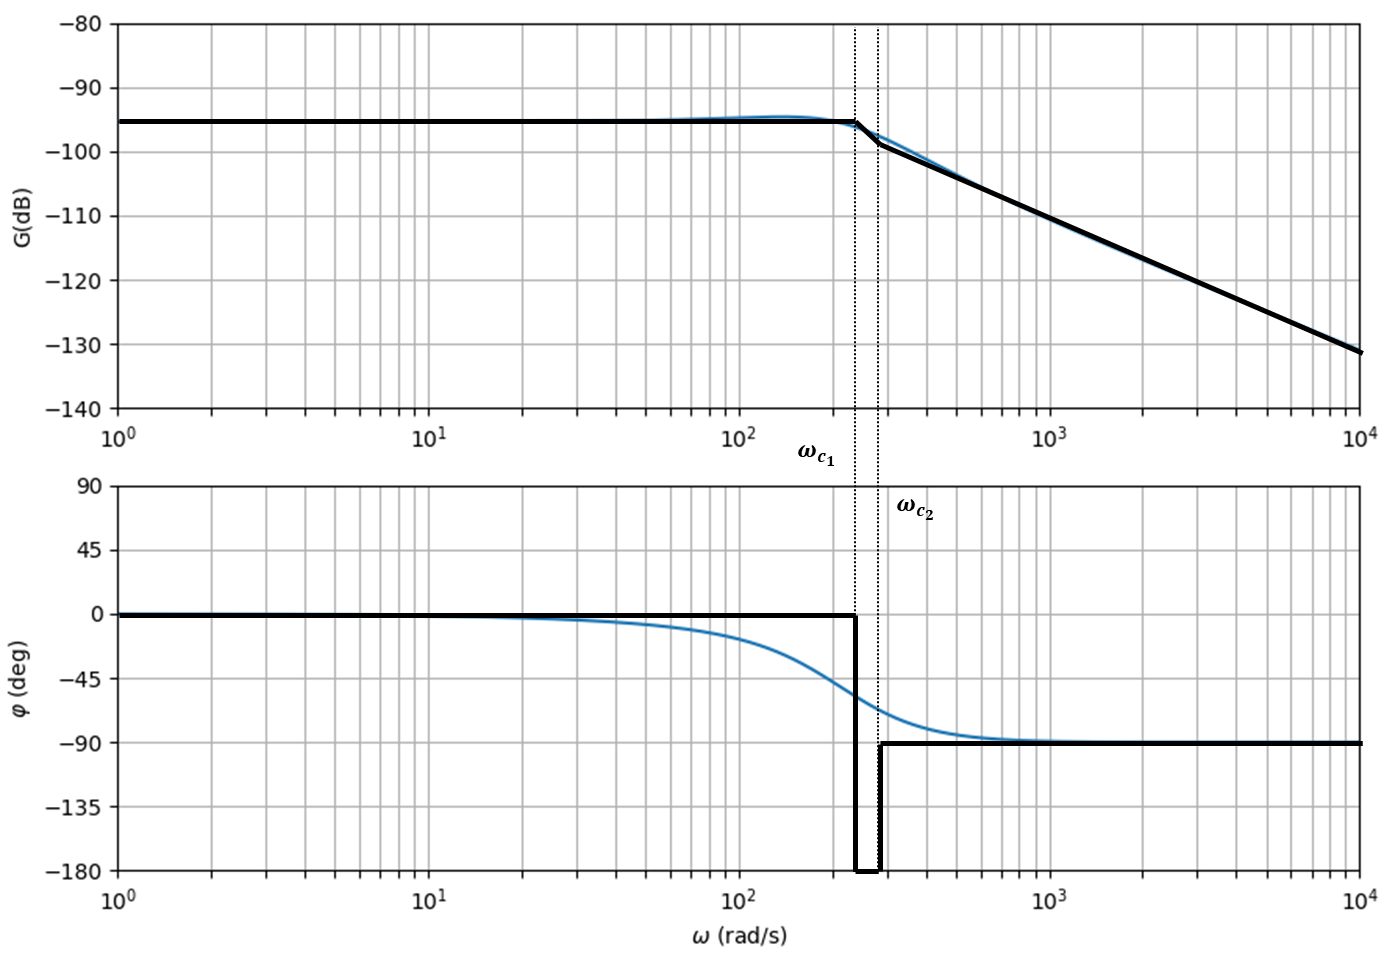
\includegraphics[width=6.15801in,height=5.58261in]{media/image4.png}

\hypertarget{iii.2---comportement-en-pente}{%
\paragraph{III.2 - Comportement en
pente}\label{iii.2---comportement-en-pente}}

La motorisation retenue permet de déplacer le robot sur sol horizontal
même en présence d'une perturbation de type frottement sec. Il faut
cependant vérifier qu'elle permet également au robot de gravir des
pentes comme indiqué dans le diagramme des exigences (Id 1.2.1), ce qui
correspond à une perturbation supplémentaire.

On se place dans le cas où le robot supporte 6 pots de masse \emph{m} =
10kg chacun. On note \emph{M} = 60kg la masse du robot. On associe au
sol le repère
\((O,\ \overrightarrow{x},\ \overrightarrow{y_{0}},\ \overrightarrow{z_{0}})\)
incliné d'un angle
\(\alpha = \left( \ \overrightarrow{y},\ \overrightarrow{y_{0}} \right) = \left( \ \overrightarrow{z},\ \overrightarrow{z_{0}} \right)\)
constant par rapport à l'horizontale.

Le robot se déplace en ligne droite selon
\((O,\ \overrightarrow{y_{0}})\) à la vitesse \emph{v}(\emph{t}), en
phase de montée. On note \emph{C\textsubscript{m}}(\emph{t}) le couple
appliqué par chaque moteur pour faire avancer le robot. Les liaisons
sont toutes supposées parfaites énergétiquement et le robot roule sans
glisser sur le sol (\textbf{figure 7}).

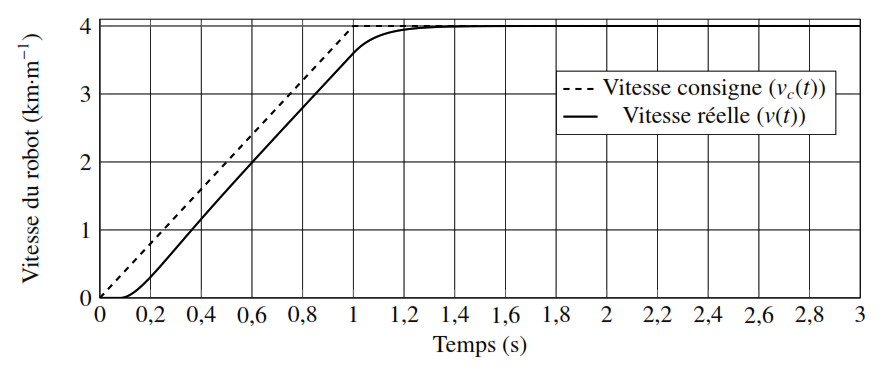
\includegraphics[width=5.36198in,height=2.58436in]{media/image5.png}

On rappelle
que\(\text{\ v}\left( t \right) = k_{t}.\omega_{m}\left( t \right)\). On
négligera l'inertie des réducteurs et des roues.

\textbf{Q12.} Montrer, en appliquant le théorème de l'énergie cinétique
au robot en mouvement, que l'équation qui décrit le mouvement du robot
en pente est la suivante :
\(M_{\text{eq}}\frac{dv(t)}{\text{dt}} = \frac{1}{r_{\text{eq}}}C_{m}\left( t \right) - F_{r,eq}\)
où l'on précisera les expressions des grandeurs équivalentes
\(M_{\text{eq}}\), \(r_{\text{eq}}\) et \(F_{r,eq}\) en fonction des
données.

Pour vérifier le dimensionnement des moteurs, on utilise les valeurs
suivantes pour les constantes déterminées précédemment :
\(M_{\text{eq}}\)≈ 120kg, \(r_{\text{eq}}\) ≈ 2·10−\textsuperscript{3}
m, \(F_{r,eq}\)≈ 200N.

On considère à nouveau la loi de pilotage définie précédemment sous
forme de trapèze avec \emph{V\textsubscript{max }}=
1,1m·s−\textsuperscript{1}, δ\emph{t} = 1s et \emph{T} = 10s.

\textbf{Q13.} Tracer l'évolution de \emph{C\textsubscript{m}}(\emph{t})
au cours du temps compte tenu de l'évolution souhaitée de
\emph{v}(\emph{t}). Préciser les valeurs caractéristiques sous forme
littérale, puis numérique.

\textbf{Q14.} À l'aide des équations du moteur, déterminer le couple
maximal développé par un moteur lorsqu'il est alimenté sous 100 V.
Vérifier alors que la motorisation est adaptée à une montée en pente du
robot.

\end{document}
